\section{Benchmark Evaluation}
\label{sec:eval}

\subsection{Experimental Design and Evidence Layers}
\label{sec:protocol}
The evaluation asks four questions: whether the governed write path rejects
predefined out-of-constraint requests, whether the five protocol stacks can be
provisioned and sampled, whether a fixed controller can close the
acquisition--actuation loop, and whether a deployed AgentTeam can convert a
production objective into governed actions. These questions are reported per
evidence unit rather than pooled into one score. Source inspection, mock
drivers, real protocol transports connected to simulated plants, and historical
LLM runs are kept separate. No physical-device or human-operator experiment is
claimed.

The primary result is the integrated archive
$B=\texttt{20260918043504-bdo}$: seed 42, commit \texttt{7d4bfc0}, harness hash
\texttt{00e7dc827f4a2cea}, Node v24.19.0 on Windows x64. It contains 75 passing
checks, no warnings, and no failures. The tool harness is the deterministic
\texttt{opencode} path; the LLM agent option is disabled. The run therefore
measures the platform, protocol, governance, fixed-controller, and AgentTeam
execution mechanisms, not model quality. The configured plants are the
cast-film physics scenario, the strategy-based film-line scenario, and the
49-signal biaxial-film full line.

\begin{table}[!t]
\centering
\caption{Evidence units in the latest integrated archive $B$. Counts refer to
checks or probes within the run and are not additional independent trials.}
\label{tab:layers}
\scriptsize
\setlength{\tabcolsep}{3.2pt}
\begin{tabular}{@{}p{0.27\columnwidth}p{0.63\columnwidth}@{}}
\toprule
Unit & Measured result \\
\midrule
Integrated run & 75/75 checks pass; 0 warnings; 0 failures \\
Protocols & Four writable lines plus one RTU satellite; 56 DAQ samples in 5/5 nodes \\
Governance & 24/24 out-of-boundary probes rejected; 0/4 designated legal writes blocked \\
Portability & Film-line: three writable lines plus two satellites; 9/9 rejected; 0/3 false blocks \\
Fixed controller & Seeds 42--44: $J/J^*=0.968$--$0.972$, mean 0.970; 6 writes total; 3/3 converged \\
AgentTeam mission & Board target $204.704\pm0.75\,^\circ$C reached with one governed write; final PV 204.700 \\
Biax full line & 9 devices, 30 setpoints and 19 acquired signals; three distinct knobs; final thickness $25.68\,\mu$m \\
Backstop & System rollback fired and restored the recorded baseline after 120.161\,s \\
HITL and recipes & Approval unblocked a suspended write; two recipe lifecycles passed \\
Platform services & Lead-to-worker task completed; duplicate memory refresh stored once; 14/14 registered engines available \\
\bottomrule
\end{tabular}
\end{table}

Safety denominators are predefined requests, not log entries or adversarial
network events. The hard-range and recipe-window probes test two specific
checks; they do not establish coverage of every fault, storage condition, or
escalation branch. Latency is reported as observed and is not treated as a
statistical equivalence result. The run is a single integrated execution, so
the reported counts are checklist coverage rather than population estimates.

\subsection{Protocol Integration and Governance}
\label{sec:port}
\label{sec:static}
\label{sec:dynamic}
\label{sec:plc}
\label{sec:govsurface}
The platform provisions Modbus TCP, OPC UA, MQTT, and HTTP as writable lines and
Modbus RTU as an acquisition-only satellite. All five nodes produce stored
samples: 7, 11, 11, 13, and 14 points, respectively. Table~\ref{tab:plc}
reports the exact write-latency and readback results. MQTT and HTTP publish or
echo without a readback value, so their accepted writes are recorded as
unverified rather than described as process confirmation.

\begin{table}[!t]
\centering
\caption{Protocol results in $B$. Write values are p50/p95 over six timed
writes; rejection is over six predefined out-of-constraint probes per stack.
RTU has no writable setpoint.}
\label{tab:plc}
\scriptsize
\setlength{\tabcolsep}{2.8pt}
\begin{tabular}{@{}lrrrr@{}}
\toprule
Stack & DAQ & p50/p95 (ms) & Readback & Reject \\
\midrule
Modbus TCP & 7 & 62.717/162.607 & $0.04\,^\circ$C & 6/6 \\
OPC UA & 11 & 18.711/21.899 & exact & 6/6 \\
MQTT & 11 & 18.837/19.140 & N/A & 6/6 \\
HTTP & 13 & 32.273/32.972 & N/A & 6/6 \\
Modbus RTU & 14 & N/A & N/A & N/A \\
\bottomrule
\end{tabular}
\end{table}

Each writable protocol rejects six probes: four engineering-range violations
and two recipe-window violations. Rejection is therefore 24/24 across the four
fixtures, and none of the four designated legal writes is blocked. This is a
coverage result for the configured probes, not a reliability estimate. The
same run provisions the independent film-line scenario with three writable
lines and two satellite nodes; its nine hard-range probes are all rejected and
its three legal writes are accepted.

The run also exercises the lifecycle around the write. Reverting a recipe
creates a new version, a known-good batch is retained, a recorded rollback
verdict does not immediately change the register, and the separately invoked
rollback executes through the write path. Manual mode suspends an agent request
until approval; the archived scripted approval releases it in 16\,ms, which is
a polling-path measurement rather than human response time. The audit surface
contains 11 parameter-change anchors for the line and returns 200-entry audit
and operations-log windows. These checks demonstrate inspectability and
separation of intent, approval, and execution; they do not turn the journal
into a cryptographically signed ledger or make asynchronous protocol I/O
atomic with recipe changes.

The process-parameter layer passes 4/4 checks. Its semantic surface exposes no
register or driver-configuration fields, writes are constrained by the
intersection of node, parameter, product, and recipe limits, an out-of-product
value is rejected, the parameter can be read back, and an unbound agent is
denied. This layer complements the node-level checks by giving operators and
agents a process-facing interface without exposing transport addresses.

\subsection{Fixed-Controller Closed-Loop Benchmark}
\label{sec:clbench}
The fixed controller starts the cast-film twin at screw speed $N=150$\,rpm,
line speed $v=95$\,m/min, and zone setpoint $200\,^\circ$C. It contains no LLM.
Its objective is
\begin{equation}
J = 55\,J_\text{thick} + 25\,J_\text{quality} +
8\,J_\text{energy} + 7\,J_\text{throughput},
\label{eq:objective}
\end{equation}
subject to melt temperature in $[195,225]\,^\circ$C and pressure at most
22\,MPa. The controller uses $N\leftarrow N(50/h)$ with a 22-rpm step limit,
holds line speed fixed, and corrects heating only when temperature leaves
$[196,224]\,^\circ$C.

\begin{figure}[!t]
\centering

\includegraphics[width=\columnwidth]{figures/publication/fig9-latest-benchmark.pdf}
\caption{Latest integrated archive $B$. (a) Protocol write latency p50/p95 for
the four writable stacks. (b) Fixed-controller objective trajectories for seeds
42--44; $J$ is sampled at the start and after each of the two governed writes.
$W^*=89.894$ is the archived finite-grid reference. The run contains 75/75
passing checks.}
\label{fig:clbench}
\end{figure}

The three seeds start at $J_0=70.115$, 68.792, and 70.248. After two governed
writes they settle at $J_{\rm end}=87.105$, 87.027, and 87.366, giving
$J_{\rm end}/J^*=0.969$, 0.968, and 0.972. All three trajectories converge,
all six writes are accepted, no write is rejected, and the mean wall time is
36.193\,s per seed. Final thicknesses are 49.883, 49.383, and
49.317\,$\mu$m; temperature and pressure stay within the stated constraints.
The reference $J^*$ is a finite-grid value, not a proven global optimum, and
the two-write count is specific to this run rather than a general bound.

\subsection{AgentTeam Optimization Mission}
\label{sec:agentloop}
The first team mission files an objective on the channel task board: bring a
Modbus-TCP temperature node to $204.704\pm0.75\,^\circ$C using at most three
governed writes after reading recent data. The lead dispatches the task, a
bound worker performs a five-minute \texttt{daq\_query}, and one
\texttt{dcw\_control} request raises the setpoint from 200 to 204.704. The
readback is 204.700, an optimization record is opened and judged
\texttt{keep}, the journal attributes the write to the agent, and the parent
task reaches \texttt{COMPLETED}; all six mission checks pass. Because the
mission policy is deterministic, this result demonstrates the task-and-tool
path rather than model-driven optimization.

The second mission is the more demanding result. The biaxial-film preset is
provisioned as one full line with nine devices, 30 writable setpoints, 19
acquired signals, and driver tests passing on all nine devices. The team files
a thickness objective of $25.0\pm0.7\,\mu$m. The initial measurement is
28.10\,$\mu$m. The worker then applies three governed, recorded actions on
three different actuator families:

\begin{enumerate}
\item cast-roll speed $32\rightarrow33.8$, thickness $28.10\rightarrow26.62\,\mu$m;
\item fast-roll speed $118\rightarrow120.5$, thickness $26.62\rightarrow25.90\,\mu$m;
\item exit rail-width setpoint $3000\rightarrow3031$, thickness $25.90\rightarrow25.68\,\mu$m.
\end{enumerate}

Each write opens a separate optimization record, returns a readback-consistent
result, is judged \texttt{keep}, and appears in the parameter ledger with agent
attribution. The final thickness is 25.68\,$\mu$m, inside the target band; the
mission records 3/6 writes, three distinct knobs, and parent-task
\texttt{COMPLETED}. Melt temperature remains at approximately
291.5\,$^\circ$C inside its 268--300\,$^\circ$C safety window.

\begin{figure}[!t]
\centering
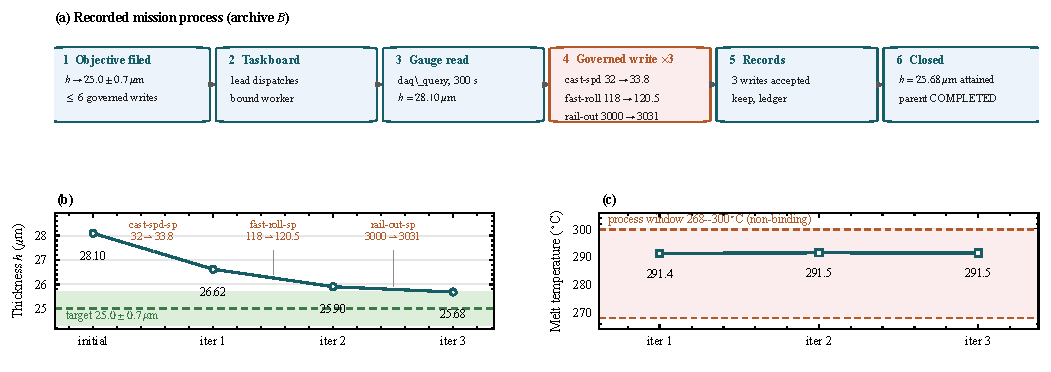
\includegraphics[width=\columnwidth]{figures/publication/fig10-agentteam-biax.pdf}
\caption{Actual AgentTeam optimization trajectory in archive $B$. The mission
reduces biaxial-film thickness from 28.10 to 25.68\,$\mu$m with three governed
writes on cast speed, fast-roll speed, and exit rail width. Every action is
read back, attributed, and judged \texttt{keep}. This deterministic
\texttt{opencode} mission tests the team and governance path, not an LLM's
optimization quality.}
\label{fig:agentteam}
\end{figure}

Figure~\ref{fig:agentteam} presents the trajectory and commands from the
machine-readable archive. The task policy is deterministic and the simulator
uses a controlled initial state, so the result should be read as an end-to-end
integration and governance test. It does not establish autonomous strategy
quality, cross-model generality, or physical-process performance.

\subsection{Governance, Reproducibility, and Boundaries}
\label{sec:e1a}
\label{sec:repro}
The backstop drill freezes a process variable outside its active window. The
system identifies an eligible open record, records a rollback judgment, and
restores the recorded baseline in 120.161\,s. This demonstrates one bounded
recovery execution; it does not exercise escalation at $K=2$ or establish a
worst-case recovery deadline. The same run stores five vector contour frames
and five image frames, completes a lead-to-worker dispatch, stores a duplicate
memory refresh once, and enumerates 14 registered and environment-available
harnesses. Registry enumeration is an inventory result, not evidence of
cross-engine control quality.

The latest archive reports a clean hard gate: 75 of 75 checks pass with no
warnings or failures. This is a reproducibility aid, not independent
replication. Deterministic structural outcomes and environment-sensitive
latencies are not interchangeable, and the run does not support a claim of
bit-identical repetition. The evidence remains simulation-tier even though the
protocol stacks are real software transports. TEP/SWaT replay, a physical
device campaign, a human-operator workload study, external-framework
comparisons, and cross-engine optimization remain unmeasured.

Historical real-LLM campaigns are retained as exploratory evidence only. They
use the same governed interface but different scoring inputs and temporal
windows; missing observations were substituted by the legacy script, and the
completion regex could match an instruction template. Those scores are
therefore not aggregated with the deterministic controller or the AgentTeam
mission. The latest $B$ report uses the deterministic team path, which avoids
blending model variability into the mechanism claims.
